围绕第 1 章确立的总体目标（式~(\ref{eq:obj})）与四个核心问题，本章依次汇报中期阶段已完成的研究进展：第~\ref{sec:dep}~节从通用计算图 $G=(O,E)$ 出发，说明如何将原始算子图化简为阶段依赖图，并结合单次 kernel 启动的硬件资源约束统一表示执行计划；第~\ref{sec:pos}~节系统对比 Persistent Kernel 与独立 Kernel 两类执行方式的优缺点与适用条件，归纳边界选择的关键硬件因素；第~\ref{sec:mech}~节介绍统一 CUDA 算子实现、基于前期工作 DACOS 的 PDL 跨边界重叠及静态启用规则；第~\ref{sec:search_sys}~节阐述基于线程块波次的耗时解析模型、引导式离线规划方法与动态 shape 自适应架构；第~\ref{sec:exp}~节在真实大模型和语料上汇报端到端与模块级实验评估结果。

\subsection{算子间依赖分析与片上资源约束建模}\label{sec:dep}\label{sec:abs}

本节回答问题一：面对输入的推理计算图 $G=(O,E)$，如何在不过度绑定特定模型的前提下完成算子间数据依赖分析，并将跨 kernel 执行决策与 GPU 片上资源约束纳入同一表示？

\subsubsection{从通用算子计算图到阶段级依赖抽象}\label{sec:form}

在第 1 章的问题建模中，系统的输入是任意推理计算图 $G=(O,E)$，其中每个节点 $o\in O$ 是一个原始算子（如矩阵乘、注意力、归一化、激活、位置编码、残差相加等）。但在实际优化时，并不需要对原始计算图里的每一条边都做“是否切分为独立 kernel”的决策。从 GPU 执行特征看，深度学习推理计算图中的算子天然分为两类：
\begin{itemize}[leftmargin=2.0em,itemsep=2pt]
\item \textbf{计算或归约主导算子}（如线性投影 GEMM、Attention 等）：计算量或访存量大，通常需要专门的矩阵分块、共享内存双缓冲和较高的寄存器预算，且不同算子偏好的线程块并行度差异显著；
\item \textbf{访存主导的轻量逐元素/尾处理算子}（如 RMSNorm、RoPE、SwiGLU/SiLU 激活、残差相加、KV 缓存写入等）：计算量极小，将它们单独拆成独立 kernel 既不能缓解寄存器或共享内存压力，反而必然带来额外的全局内存读写和 kernel 启动开销。
\end{itemize}

基于这一共性规律，本课题对任意输入计算图 $G=(O,E)$ 首先执行一道\textbf{与具体模型无关的轻量算子吸收（prologue/epilogue 预融合）}：将轻量逐元素与尾处理算子直接并入相邻主导算子的输入准备或输出收尾阶段，从而把原始算子图 $G=(O,E)$ 化简为由主导计算阶段构成的\textbf{阶段依赖图} $G_S=(V_S,E_S)$。真正存在“融合为同一 kernel”与“切分为独立 kernel”硬件权衡的，正是阶段图中的相邻阶段边 $e=(u,v)\in E_S$。需要强调的是，这套从 $G=(O,E)$ 到 $G_S=(V_S,E_S)$ 的化简与建模方法并不局限于某一种特定网络：若换成 Qwen、Gemma、Mistral 等不同归一化或激活形式的模型，或是包含路由与专家分组 GEMM 的 MoE 模型、多头潜在注意力（MLA）及混合架构，化简后仅是阶段图 $G_S$ 的节点类型与连接关系随之变化，后续的依赖分析、资源约束建模、PDL 重叠和方案搜索流程均直接作用在 $G_S$ 上，无需针对单一模型硬编码固定阶段数。

在中期真机实验验证中，课题以主流轻量化模型 Llama-3.2-1B（16 个解码层，隐藏维度 2048，中间层维度 8192，32 个查询头与 8 个键值头）作为具体实例。将上述通用化简规则作用于 Llama 解码层后，每层自然归结为五个顺序主导阶段：Q 阶段（输入 RMSNorm、QKV 线性投影、RoPE 位置编码与 KV cache 写入）、A 阶段（attention 计算）、O 阶段（输出投影、残差相加与后继 RMSNorm）、U 阶段（gate/up 投影并在寄存器内融合 SwiGLU 激活）以及 D 阶段（down 投影、残差相加与下一层输入 RMSNorm）；全模型首层前接词嵌入（embedding），末层后接词表投影与贪心采样（argmax）。层内与跨层相邻阶段由此构成五类核心算子边：Q$\to$A、A$\to$O、O$\to$U、U$\to$D 以及跨层边 D$\to$Q。

对应第 1 章中的任务级依赖分析，对阶段图中的任意依赖边 $e=(K_i,K_j)\in E_S$，系统同时分析两方面信息：一是\textbf{数据就绪粒度}，即后继 $K_j$ 的某个任务是仅需前驱局部输出即可开始（局部就绪），还是必须等待前驱全部输出完成（全量就绪）；二是沿用前期工作 DACOS~\pDacos 对跨 kernel 输入的划分，将后继 $K_j$ 的输入拆分为前驱实时产出的\textbf{依赖张量}与启动时刻即已就绪的\textbf{独立张量}（如只读权重、张量描述符与索引元数据），进而提取出可在首次读取依赖数据前合法提前执行的\textbf{独立前缀}。表~\ref{tab:edges} 给出了 Llama-3.2-1B 实例下五类阶段边的依赖形态与独立前缀。

\begin{table}[!htb]\centering
\caption{Llama-3.2-1B 解码层实例中五类相邻阶段边的依赖就绪形态与消费者独立前缀}\label{tab:edges}
\small
\begin{tabularx}{\textwidth}{@{}p{1.4cm}>{\raggedright\arraybackslash}p{6.5cm}>{\raggedright\arraybackslash}X@{}}
\toprule
算子边 & 数据依赖就绪形态 & 消费者可提前执行的独立前缀\\
\midrule
Q$\to$A & 局部就绪：各 KV 头分组的 attention 仅依赖对应头的 Q、K、V 输出 & 历史缓存 KV 块的异步读取（decode 阶段）\\
A$\to$O & 全量就绪：输出投影的每个分块均依赖全部查询头的完整聚合结果 & 输出投影权重（8\,MiB）的片外预取\\
O$\to$U & 全量就绪：每个输出分块依赖前驱在对应 token 行上的完整归一化输出 & Gate/up 投影权重（64\,MiB）的片外预取\\
U$\to$D & 全量就绪：down 投影沿中间维度归约，依赖完整的激活张量 & Down 投影权重（32\,MiB）的片外预取\\
D$\to$Q & 全量就绪：下一层 QKV 投影依赖完整的层间归一化激活 & 下一层 QKV 权重（12\,MiB）的片外预取\\
\bottomrule
\end{tabularx}
\end{table}

对应第 1 章定义的边级候选空间 $\mathcal{M}(e)$，阶段图中的每条边 $e\in E_S$ 可选用三类物理执行方式（图~\ref{fig:scheme}）：
\begin{enumerate}[leftmargin=2.4em,itemsep=2pt]
\item \textbf{同 grid 融合}：将前后阶段编译进同一个 persistent grid，靠设备端全局屏障保证全局内存可见；
\item \textbf{跨 grid completion（串行切分）}：在该边切分为两个独立 kernel，等待前驱全部线程块退出后再启动后继；
\item \textbf{跨 grid PDL（切分并重叠）}：保留物理切分边界，由前驱在尾部发出 programmatic completion 信号提前启动后继，让后继先执行独立前缀再等待前驱数据就绪。
\end{enumerate}

针对开题提到的“同 grid 细粒度事件”形态，课题前期也在 Hazy Megakernels 原型\pHazy 上做了对比测试：在 1024 上下文单请求 decode 中，为 QKV 保留按头局部就绪、为 gate/up 采用全量就绪的混合配置可比逐边贪心缩短 11.4--12.7\us（1136.3\us）；但同一原型上的对照同时表明，若各阶段线程块和资源配置保持不变、单纯把单 kernel 拆成多 kernel，时延反而升至 1185.6\us，只有同步重新配置切分后各组的资源参数，PDL 才能把粗粒度切分从串行的 1419.1\us 压低至 1291.9\us。这一现象说明：\textbf{是否切分某条算子边不能脱离硬件资源配置孤立决定，必须与 GPU 单次 kernel 启动的片上资源约束联合建模。}

\begin{figure}[!htb]\centering
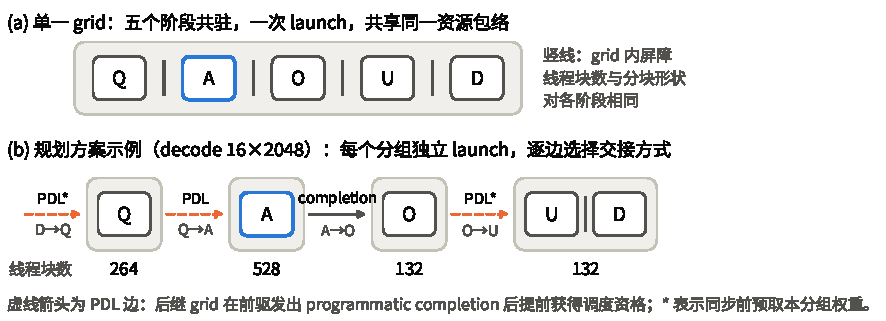
\includegraphics[width=\textwidth]{Img/midterm/scheme}
\caption{阶段依赖图及其边级执行映射示例。(a) 单一 persistent grid 方案下，五个阶段通过核内屏障顺序衔接，共享同一套寄存器与共享内存上限；(b) 针对 decode 16$\times$2048 选出的混合执行计划：attention 独立成组并扩展至 528 个线程块，U 与 D 保持同 grid 融合，四条物理边界中有三条启用跨边界 PDL 重叠。}\label{fig:scheme}
\end{figure}

\subsubsection{单次 Kernel 启动的资源约束与全图执行计划表示}\label{sec:env}

从 GPU 硬件执行模型看，每个线程占用的寄存器数量和每个线程块占用的共享内存大小，都是以\textbf{单次物理 kernel 启动（launch）}为粒度在编译和启动时静态锁定的。当多个连续阶段被融合进同一个物理 grid $g$ 时，整个 kernel 必须按组内需求最苛刻的阶段来分配片上资源：
\begin{equation}
r(g)\ge\max_{s\in g} r_s,\qquad m(g)=\max_{s\in g} m_s. \label{eq:env}
\end{equation}
设单个流多处理器（SM）的寄存器文件容量为 $R_{\mathrm{SM}}$、共享内存容量为 $M_{\mathrm{SM}}$、最大常驻线程数为 $T_{\mathrm{SM}}$（NVIDIA H100 上分别为 65\,536、228\,KiB 与 2048），每线程块包含 $\tau=128$ 个线程时，单个 SM 最多能同时驻留的线程块数 $n(g)$（即 occupancy 上限）由三者中的最小值决定：
\begin{equation}
n(g)\le\min\Bigl(\Bigl\lfloor\frac{R_{\mathrm{SM}}}{\tau\, r(g)}\Bigr\rfloor,\ \Bigl\lfloor\frac{M_{\mathrm{SM}}}{m(g)}\Bigr\rfloor,\ \Bigl\lfloor\frac{T_{\mathrm{SM}}}{\tau}\Bigr\rfloor\Bigr), \label{eq:occ}
\end{equation}
使用协作启动（cooperative launch）时，全卡同时运行的总线程块数不得超过 $n(g)$ 与设备 SM 总数（132）之积。

据此，第 1 章式~(\ref{eq:obj}) 中的全图执行计划 $\Pi$ 在阶段图 $G_S=(V_S,E_S)$ 上可以明确写为三元组 $\Pi=\langle C,\allowbreak \{\theta_g\},\allowbreak \{\varphi_e\}\rangle$：其中 $C\subseteq E_S$ 为切分为物理 kernel 边界的边集合（切分后将阶段图划为若干连续分组 $g$；在 Llama 每层五类边同构取值下共有 $2^5=32$ 种切分方案，$C=\varnothing$ 即退化为全图单一 persistent kernel）；$\theta_g$ 为分组 $g$ 的执行配置，包含矩阵分块形状、启动线程块数及核内各阶段活跃块配置；$\varphi_e\in\{\text{completion},\allowbreak \text{PDL},\allowbreak \text{PDL}^*\}$ 为物理边界 $e\in C$ 的跨核衔接方式（$\text{PDL}^*$ 表示等待前驱数据前附带静态权重预加载）。

\subsection{Persistent Kernel 与独立 Kernel 的优缺点剖析及边界选择因素}\label{sec:pos}

在统一建模的基础上，本节回答问题二：全图融合（Persistent Kernel）与独立切分（Split Kernel）各自的优势和瓶颈究竟在哪里？为什么不同算子边界、不同输入规模需要选择不同的执行方式？

\subsubsection{Persistent Kernel 的优势与资源耦合瓶颈}\label{sec:hw}

Persistent Kernel 将多个连续计算阶段甚至整网融合进同一个物理 grid，整次前向只需启动一次 kernel，常驻 SM 的线程块之间通过设备端同步屏障衔接。它的核心优势非常直接：\textbf{完全消除了主机侧反复提交 kernel 的开销，也避免了相邻 kernel 之间“等待前驱全部退出再重新启动后继”的空闲间隙}。因此，当各阶段所需的线程块数与片上资源需求比较接近时，单一 persistent kernel 确实最快。如表~\ref{tab:cores} 所示，在单请求短上下文 decode（$1\times 512$）和采用轻量逐 warp attention 的极短 prefill（$1\times 16$）上，五阶段融合执行的单层耗时比五阶段各自独立最优之和分别还快 1.3\us 和 1.8\us。

然而，一旦进入长上下文、中大批量或重度算子区间，单一 persistent kernel 就会明显变慢。慢的原因是什么？我们首先通过图~\ref{fig:hw} 的受控微基准排除了“同步原语开销”的猜测：放进 CUDA Graph 封装后~\pGraph，两个空阶段之间无论是用核内全局屏障、跨 grid 串行 completion 还是跨 grid PDL，132 个线程块下的单次同步耗时都在 1.16\us 左右，扩展到 528 块也仅在 1.40--1.88\us 之间（图~\ref{fig:hw}(a)）；同时，流式读取 64\,MiB 线性权重在 264 个线程块（每 SM 2 块，6 级异步流水）处就已吃满 H100 的 HBM 带宽（2.4--3.0\,TB/s，图~\ref{fig:hw}(b)）。这说明，单一 persistent kernel 变慢的真正根源并非同步本身，而是式~(\ref{eq:env})--(\ref{eq:occ}) 揭示的\textbf{不同阶段共享同一片上资源上限造成的冲突}。

\begin{figure}[!htb]\centering
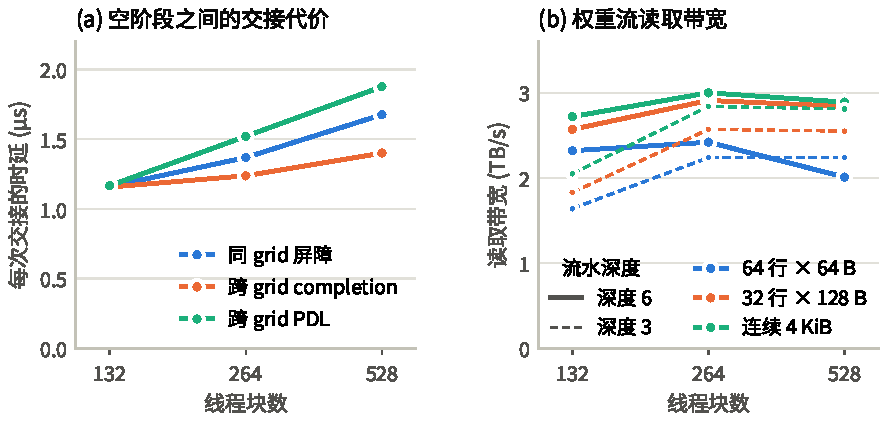
\includegraphics[width=\textwidth]{Img/midterm/hw_micro}
\caption{跨阶段同步开销与流式权重读取带宽微基准。(a) 相邻空阶段间三种衔接方式随线程块数的单次耗时；(b) 流式读取 64\,MiB gate/up 权重的有效带宽随线程块数与访存连续性的变化，在 264 个线程块处即达到平台带宽上限。}\label{fig:hw}
\end{figure}

具体到线性矩阵阶段（Q、O、U、D）与 attention 阶段（A），二者在理想线程块数与片上资源占用上存在两重明显矛盾（图~\ref{fig:stage} 与表~\ref{tab:foot}）：
\begin{enumerate}[leftmargin=2.4em,itemsep=2pt]
\item \textbf{最优线程块并行度相反。}四个矩阵阶段独立运行时普遍在 132 或 264 个线程块处最快，继续增加线程块反而加剧缓存竞争与归约成本；而高负载 decode attention 随线程块数增加显著提速（例如 $16\times 2048$ 下 528 块比 132 块快 2.5 倍）。
\item \textbf{寄存器与共享内存互相拖累。}在 decode 中，矩阵阶段每块需要 72\,KiB 共享内存，将五阶段融合 kernel 的单 SM 并发上限压在 3 块（全卡 396 块），使原本能跑 4 块/SM（528 块）的 attention 损失了四分之一并发度；在 prefill 中，基于 Tensor Core 的 FlashAttention-2~\pFA 每线程用满 255 个寄存器，一旦与矩阵阶段融合，全图所有阶段的并发度都会被拉低到每 SM 2 块（264 块）。
\end{enumerate}

\begin{figure}[!htb]\centering
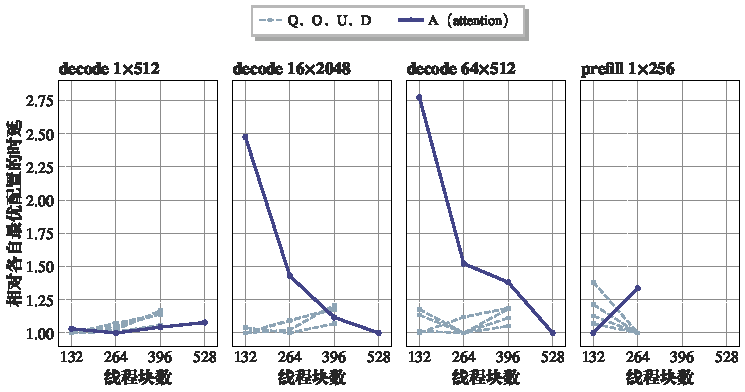
\includegraphics[width=\textwidth]{Img/midterm/stage_ctas}
\caption{矩阵阶段与 attention 阶段独立运行时的最优线程块并行度差异。纵轴为归一化至各阶段最优配置的相对时延；矩阵阶段偏好 132--264 个线程块，而高负载 decode attention 随线程块数扩展至 528 持续提速。}\label{fig:stage}
\end{figure}

\begin{table}[!htb]\centering
\caption{各阶段独立编译与五阶段融合时的静态片上资源需求对比。寄存器按每线程计，共享内存（KiB）按每线程块计，“块/SM”为协作启动单 SM 最大并发线程块数}\label{tab:foot}
\footnotesize\setlength{\tabcolsep}{4.5pt}
\begin{tabular}{@{}lccc@{\hspace{1.4em}}ccc@{\hspace{1.4em}}ccc@{}}
\toprule
 & \multicolumn{3}{c}{Decode（128$\times$16）} & \multicolumn{3}{c}{Prefill，FA2（64$\times$64）} & \multicolumn{3}{c}{Prefill，逐 warp（64$\times$64）}\\
\cmidrule(r{1.4em}){2-4}\cmidrule(r{1.4em}){5-7}\cmidrule{8-10}
阶段或分组 & 寄存器 & KiB & 块/SM & 寄存器 & KiB & 块/SM & 寄存器 & KiB & 块/SM\\
\midrule
Q 阶段 & 124 & 72 & 3 & 158 & 64 & 3 & 158 & 64 & 3 \\
A 阶段 & 124 & 16 & 4 & 255 & 48 & 2 & 48 & 0 & 4 \\
O 阶段 & 122 & 72 & 3 & 150 & 64 & 3 & 150 & 64 & 3 \\
U 阶段 & 112 & 72 & 3 & 144 & 64 & 3 & 144 & 64 & 3 \\
D 阶段 & 122 & 72 & 3 & 150 & 64 & 3 & 150 & 64 & 3 \\
五阶段融合 & 162 & 72 & 3 & 255 & 64 & 2 & 168 & 64 & 3 \\
\bottomrule
\end{tabular}
\end{table}

为了定量衡量这种资源冲突带来的损失，定义单层\textbf{共驻代价}为“五阶段融合在最优单一 grid 中的单层耗时”减去“五阶段各自独立成组并分别取最优配置时的耗时之和（已包含独立启动开销）”。表~\ref{tab:cores} 清楚显示：在重载 decode（$+10.2$ 至 $+21.4$\us/层）、含 FlashAttention-2 的 prefill（$+13.7$ 至 $+40.6$\us/层）以及不同矩阵阶段偏好不同分块的中等规模 prefill（$16\times 16$ 下达 $+25.2$\us/层）上，强行融合付出的资源受限代价远高于微秒级的跨 kernel 启动开销。

\begin{table}[!htb]\centering
\caption{单层耗时分解与融合共驻代价实测对比（\textmu s）。共驻代价为正表示多阶段共享片上资源上限带来的损失超过独立切分的启动开销}\label{tab:cores}
\footnotesize\setlength{\tabcolsep}{4.5pt}
\begin{tabular}{@{}lrrrrrrrr@{}}
\toprule
典型负载 & Q & A & O & U & D & 独立最优之和 & 五阶段融合 & 共驻代价\\
\midrule
decode 1$\times$512 & 9.9 & 8.3 & 11.0 & 26.2 & 19.6 & 75.0 & 73.7 & $-1.3$ \\
decode 4$\times$8192 & 10.1 & 41.9 & 11.0 & 26.4 & 19.7 & 109.1 & 119.4 & $+10.2$ \\
decode 16$\times$2048 & 10.5 & 41.0 & 11.0 & 26.7 & 20.1 & 109.4 & 120.0 & $+10.6$ \\
decode 64$\times$512 & 13.0 & 39.0 & 11.4 & 28.6 & 22.7 & 114.7 & 136.1 & $+21.4$ \\
prefill 1$\times$16（逐 warp） & 10.6 & 7.3 & 11.1 & 27.0 & 20.3 & 76.3 & 74.5 & $-1.8$ \\
prefill 1$\times$16（FA2） & 10.6 & 7.8 & 11.1 & 27.0 & 20.2 & 76.7 & 90.4 & $+13.7$ \\
prefill 1$\times$256（FA2） & 23.4 & 11.8 & 16.5 & 52.8 & 34.9 & 139.4 & 179.9 & $+40.6$ \\
prefill 16$\times$16（逐 warp） & 23.4 & 19.2 & 16.4 & 52.7 & 34.6 & 146.3 & 171.5 & $+25.2$ \\
\bottomrule
\end{tabular}
\end{table}

\subsubsection{独立 Kernel 切分的收益与算子间等待及重叠限制}\label{sec:split}

与全图融合相反，将计算图切分为独立物理 kernel 的核心优势在于\textbf{解除片上资源耦合}：切分后每个阶段分组各自独立编译与启动，矩阵阶段和 attention 阶段都能按自身特点选择最合适的分块形状、寄存器预算和线程块数。但是，独立切分同样面临两方面突出局限：

\textbf{局限一：串行执行导致算子间等待间隙沿执行链累积。}在传统的 completion 语义下，必须等前驱 kernel 的最后一个线程块完全退出，GPU 才会启动后继 kernel。正如前期工作 DACOS~\pDacos 在短序列 LLM 工作流中指出的，尽管后继算子包含描述符初始化、只读权重加载等不依赖前驱输出的操作，严格的串行边界仍使相邻 kernel 间的等待与启动间隙逐层叠加：16 层五阶段全切分共有 79 个物理边界，在 decode $1\times 512$ 上累计产生 166\us 间隙（约占总时延的 11\%），导致资源冲突较轻的中小批量负载单纯切分反而比单一 persistent kernel 慢 1.4\%--5.4\%。

\begin{figure}[!htb]\centering
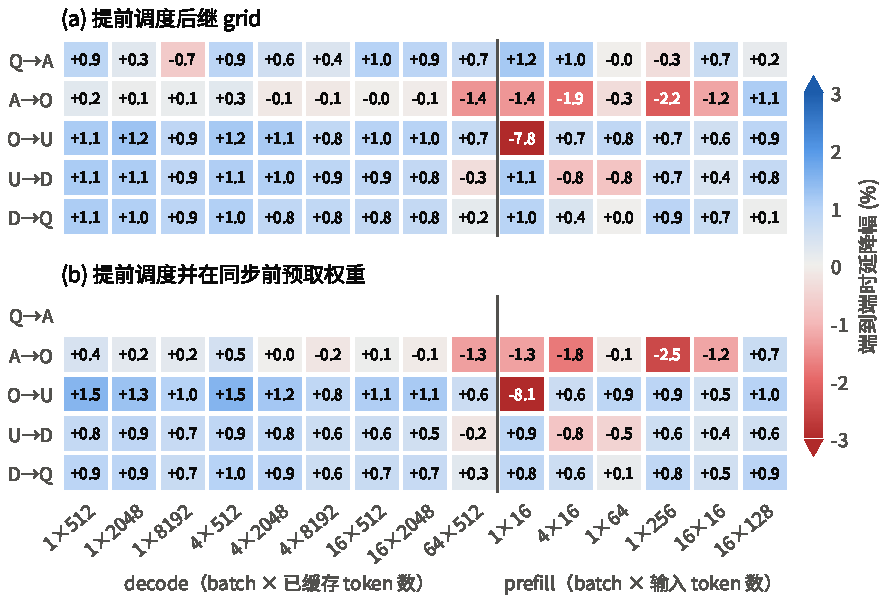
\includegraphics[width=\textwidth]{Img/midterm/pdl_edges}
\caption{五阶段全切分下各类物理边界单独启用 PDL 或带预取 PDL* 相对串行 completion 的端到端时延降幅（正值表示加速）。Q$\to$A 后继为无静态权重的 attention 阶段；色标截断于 $\pm 3\%$，格内标注实测百分比。}\label{fig:pdl}
\end{figure}

\textbf{局限二：借助硬件 PDL 提前启动后继，在异构切分图上并非总能获益。}Hopper 架构提供了硬件级 PDL 机制~\pPDL，允许后继在前驱尚未完全退出时提前启动以隐藏上述间隙。但图~\ref{fig:pdl} 在五阶段全切分上逐边实测的结果表明，PDL 的效果高度分化：decode 中以矩阵为后继的四类边在 36 组仅提前启动测试中有 34 组稳定提速（叠加权重预取最高达 $+1.5\%$）；而在 prefill 中，A$\to$O 边在 5 个负载上均变慢（$-0.3\%$ 至 $-2.2\%$），$1\times 16$ 下的 O$\to$U 边甚至出现 $-7.8\%$ 的明显倒退。在 decode $16\times 2048$ 的全部 31 种切分方案中，对所有物理边界盲目开启 PDL 有 27 种反而慢于纯串行执行。

\subsubsection{边界执行机制的决定因素、相关工作局限与本文思路}\label{sec:factors}

将视野扩展到动态输入规模，如图~\ref{fig:motiv} 所示，15 个覆盖不同 batch 和序列长度的 decode 与 prefill 负载最终分化出 11 种不同的最优逐边执行方案——全图单一 persistent kernel、固定全切分串行、固定全切分全局 PDL 都无法覆盖全部区间。综合上述实测可以清楚地回答问题二：\textbf{一条算子边界应当融合还是切分、切分后是否启用 PDL，由三类可量化的硬件因素共同决定}：
\begin{enumerate}[leftmargin=2.4em,itemsep=2pt]
\item \textbf{两侧阶段的融合资源代价}：融合后因共享寄存器、共享内存和线程块数带来的额外耗时是否高于单次跨 kernel 启动开销（决定该边是融合还是切分）；
\item \textbf{物理边界两侧的共享内存配置兼容性与 SM 剩余资源}：决定 PDL 后继线程块能否顺利提前进入正在执行前驱的 SM，还是被挡在外面、集中挤入最先空闲的少数 SM 引发负载不均；
\item \textbf{后继的 L1 缓存敏感度与前驱尾部的 HBM 带宽余量}：决定提前进入是否因共享内存配置沿用导致 L1 缓存缩水，以及权重预加载是否与前驱争夺 HBM 带宽。
\end{enumerate}

\begin{figure}[!htb]\centering
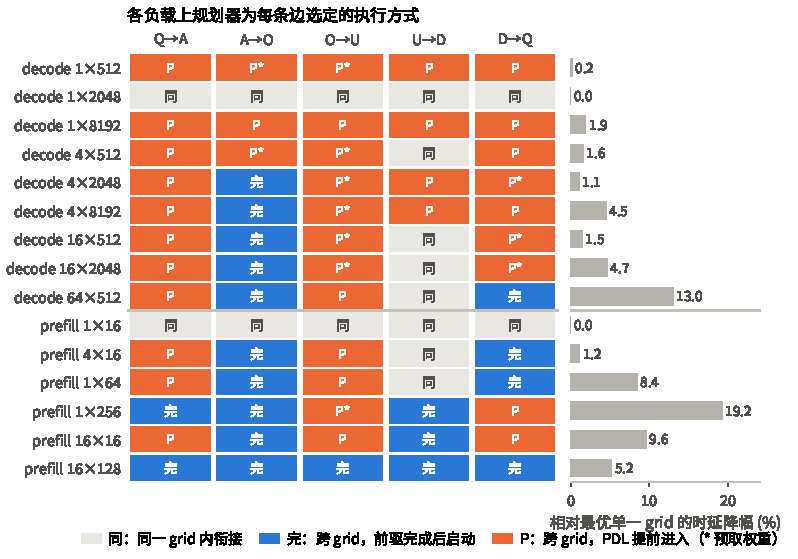
\includegraphics[width=0.9\textwidth]{Img/midterm/motiv_edges}
\caption{15 个典型负载上最优逐边执行方案的分化特征及其相对最优单一 grid 的时延降幅。}\label{fig:motiv}
\end{figure}

对照这三类因素审视现有相关工作，可以看出三点不足：第一，全图单一 kernel 方案（Hazy Megakernels\pHazy、MPK\pMPK）以全融合为既定目标，无法消除异构阶段间的寄存器与共享内存冲突，近期拆解分析~\pQiang 与编译器实践~\pcite{together2026}{Together AI，2026}也证实核内屏障（约 646\,ns）与 CUDA Graph 配合 PDL 的边界开销（约 645\,ns）几乎一致，强行融合反而变慢；第二，现有融合与动态 shape 编译方法多聚焦于单 kernel 内部优化~\pcite{zhengz2022}{Zheng 等，2022a}、静态配置（\rcite{nvidiate}{NVIDIA，2026g}；\rcite{andoorveedu2026}{Andoorveedu 等，2026}）或粗粒度区段切换（\rcite{chatterjee2026}{Chatterjee 等，2026a}；\rcite{chatterjee2026b}{Chatterjee 等，2026b}），而动态 shape 微内核编译如 MikPoly~\pcite{yu2024}{Yu 等，2024} 与 MoonPoly~\pcite{zhangy2026}{Zhang 等，2026a} 仅调节算子内分块参数，算子间仍固定串行启动；第三，在跨 kernel 重叠限制方面，既有记录仅在多流并发下零星观察到共享内存配置干扰（\rcite{nvidiaforum}{NVIDIA，2025}；\rcite{strati2026}{Strati 等，2026}；\rcite{flashinfer7548}{FlashInfer，2026}）或寄存器受限~\pQiang，前期工作 DACOS~\pDacos 也仍以固定算子边界为前提。

因此，本课题的核心思路是：\textbf{不再预设全融合或全切分，而是把阶段图每条边的执行方式提升为决策变量，与各分组的资源配置和硬件调度规律协同求解。}下面两节分别阐述执行机制实现（2.3 节）以及低开销规划与动态 shape 适配方法（2.4 节）。

\subsection{自适应执行机制设计与实现}\label{sec:mech}

围绕问题三，本节首先说明如何在同一套 CUDA 代码上公平实现任意阶段融合与核内分阶段并发控制（2.3.1 节），随后结合前期工作 DACOS 的 PDL 重叠框架剖析 H100 上跨边界重叠的两项底层硬件规律（2.3.2 节），最后导出无需逐边真机试错的静态 PDL 启用规则（2.3.3 节）。

\subsubsection{统一 CUDA 算子实现与核内分阶段并发控制}\label{sec:method}

为了排除外部算子库实现差异、保证不同切分方案在完全一致的算子代码下对比运行，课题实现了一套模板化统一 CUDA 后端：从词嵌入、解码层五个阶段到末层贪心采样共享同一套设备端代码，任意连续阶段区间都可以编译实例化为独立的协作式 persistent grid。具体算子实现上，矩阵阶段提供 $64\times 64$、$128\times 64$ 与 $128\times 16$（列 $\times$ 行）三种 Tensor Core 分块形状，支持沿归约维（K 维）切分，并在收尾融合残差、RMSNorm、RoPE 与 KV 写入；decode attention 采用按历史键值切片并行与双缓冲异步加载的在线归约实现（较早期逐键串行提速 1.1--2.0 倍），prefill attention 同时提供 FlashAttention-2 与零共享内存的逐 warp 在线归约两种实现。

同时，针对多阶段融合在同一个 persistent grid 内时“矩阵偏好 132--264 块、attention 偏好更多块”的内部矛盾，后端引入了\textbf{按物理 SM 重排逻辑块号的核内分阶段活跃块控制}。kernel 启动初期，每个线程块读取硬件寄存器 \texttt{\%smid} 并通过原子计数按“同 SM 内块序号优先、物理 SM 编号次之”重新分配逻辑块号，确保任意前缀子集都能均匀分布到全卡 132 个 SM 上。借此，同一个 persistent kernel 内的矩阵阶段只激活每 SM 1--2 个线程块以保持缓存效率与整波对齐，而 attention 阶段激活全部常驻线程块以充分并行，其余休眠块仅参与轻量屏障同步。实测表明，这一控制让单一 grid 基线自身在 decode $16\times 2048$ 上先提速 6.0\%（由 2201.8\us 降至 2070.8\us），保证了后续所有切分对比都建立在公平的强单核基线之上。

\subsubsection{基于 DACOS 的 PDL 跨边界重叠与 SM 调度规律}\label{sec:pdl}\label{sec:admit}\label{sec:place}

针对物理切分后的算子边界，本课题沿用并拓展了前期已发表工作 DACOS~\pDacos 的依赖感知跨 kernel 重叠框架（图~\ref{fig:dacos}）。DACOS 面向短序列大模型推理中频繁的算子间等待问题，通过三部分机制把相邻 kernel 之间的空闲间隙转化为有效准备与数据预加载：
\begin{enumerate}[leftmargin=2.4em,itemsep=2pt]
\item \textbf{跨 kernel 依赖分析与重叠阶段构造。}对相邻 kernel 依赖边 $(K_i, K_j)$，将后继 $K_j$ 的输入拆分为依赖张量与独立张量，以首次读取依赖张量的同步点——\textbf{依赖前沿} $\mathcal{F}(K_j)$（对应 \texttt{cudaGrid\allowbreak{}Dependency\allowbreak{}Synchronize()}）——为界，把后继拆分为依赖无关的重叠准备阶段与依赖主体 $K_j = K_j^{\mathrm{overlap}} \cup K_j^{\mathrm{dep}}$。其中 $K_j^{\mathrm{overlap}}$ 在前驱尚未结束时即可完成索引与指针计算、张量描述符构建、独立张量向 L2 缓存或共享内存的预加载（如 GEMM 权重预载或 Attention 的 Q 分块预载）及辅助状态初始化。
\item \textbf{三维重叠配置空间与成对代价模型。}前驱 $K_i$ 在可调预启动时机 $\tau_i$ 调用 \texttt{cudaTrigger\allowbreak{}Programmatic\allowbreak{}Launch\allowbreak{}Completion()} 暴露重叠窗口 $W_i(\tau_i)$，后继在由预启动时机 $\tau_i$、预加载数据量 $s_i$ 与存储层级位置 $h_i \in \{\text{L2},\text{SHM},\text{REG}\}$ 构成的配置空间 $\theta_i = \langle \tau_i, s_i, h_i \rangle$ 中择优。DACOS 通过成对代价模型评估重叠执行后的联合时延：
\begin{equation}
\begin{aligned}
\hat{L}_{i,j}(\theta_i) &= T^{\mathrm{base}}(K_i)+T^{\mathrm{dep}}_j+\max\!\bigl(0,\,T^{\mathrm{overlap}}_j(\theta_i)-W_i(\tau_i)\bigr)\\
&\quad -G^{\mathrm{residency}}_i(\theta_i)+P^{\mathrm{cache}}_i(\theta_i),
\end{aligned}
\label{eq:dacos}
\end{equation}
定量权衡超出重叠窗口的未隐藏开销、数据提前驻留收益 $G^{\mathrm{residency}}_i$ 与缓存干扰惩罚 $P^{\mathrm{cache}}_i$。
\item \textbf{参数化模板与运行时实例化。}借助参数化 PDL 内核模板（KPT）和输入形状分桶缓存，DACOS 在运行时为不同输入形状选择最优 $\theta_i^\star$ 并填充启动描述符。在真实短序列 LLM 负载上，DACOS 相对 TorchEager 与 TorchInductor 最高分别取得了 $3.5\times$ 与 $1.2\times$ 的端到端加速。
\end{enumerate}

\begin{figure}[!htb]\centering
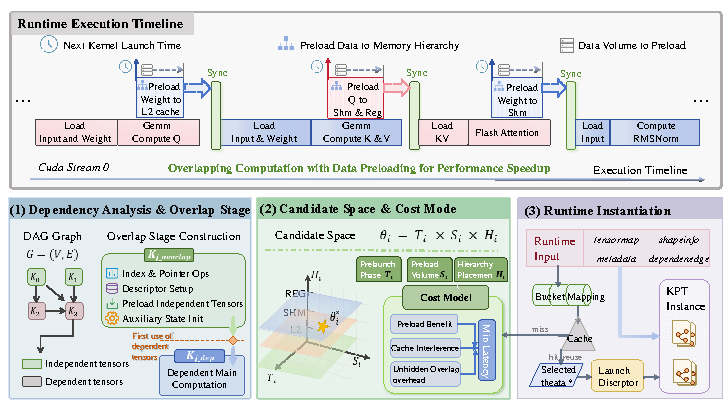
\includegraphics[width=\textwidth]{Img/midterm/dacos_overview}
\caption{前期工作 DACOS~\pDacos 的依赖感知跨 kernel 重叠框架与运行时执行时间线。上方展示在单一 CUDA Stream 中通过 PDL 提前启动后继并将权重/Q 分块预加载至 L2、共享内存或寄存器的重叠过程；下方依次为依赖分析与重叠阶段构造、三维配置空间与代价模型、以及基于形状分桶缓存的运行时实例化流程。}\label{fig:dacos}
\end{figure}

把 DACOS 框架拓展到本课题的可变分组切分图上时，H100 实测进一步揭示了两项此前未被充分刻画的底层硬件限制，正是它们解释了第~\ref{sec:split}~节（图~\ref{fig:pdl}）中部分边开启 PDL 反而变慢的原因：

\textbf{第一，HBM 带宽余量限制了连续矩阵链上的预加载量。}在 H100 受控带宽测试中，如果前驱是不占 HBM 带宽的纯算术负载，仅提前启动后继可省 0.1--0.3\us，叠加 8\,MiB 权重预加载凭借 L2 驻留可将收益放大到 1.0--1.4\us（32--64\,MiB 饱和于 1.5\us）；但当链路是持续打满 HBM 带宽的连续矩阵阶段时，仅提前启动能稳定隐藏 0.4--0.8\us 启动间隙，叠加 1\,MiB 预加载净收益降至 0.2--0.5\us，预加载 8\,MiB 以上则会与前驱抢占 HBM 带宽反而倒退 0.8--7.3\us（真实模型 21 组全切分测试中，1\,MiB 预加载相对纯提前启动的中位变化为 $-0.20$\us 至 $+0.12$\us）。因此，本课题的统一模板将带宽密集链上的重叠前缀限定为轻量初始化与至多 1\,MiB 权重预加载。

\begin{figure}[!htb]\centering
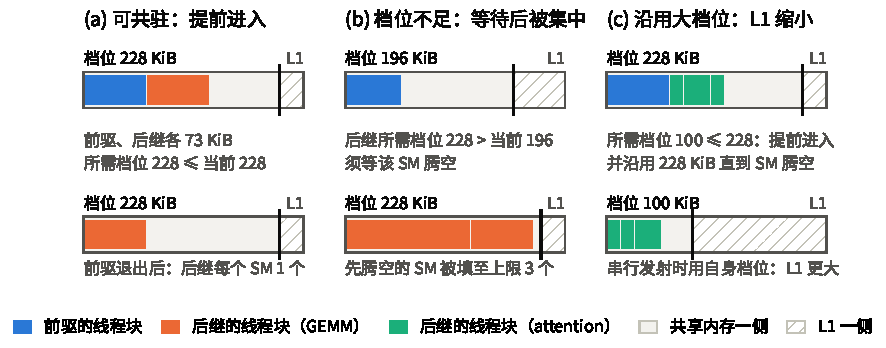
\includegraphics[width=\textwidth]{Img/midterm/v4_carve}
\caption{共享内存 carve-out 配置档位决定的三种 PDL 调度情形。横条表示单个 SM 的统一片上存储，竖线左侧为共享内存、右侧为 L1 缓存：(a) 后继所需档位不高于当前档位且剩余资源充足，顺利提前进入 SM 并发执行；(b) 后继需求档位高于当前档位，被迫等待部分 SM 空闲并集中调度到先空闲的少数 SM；(c) 需求档位较低的后继提前进入后被动沿用前驱大档位，导致可用 L1 缓存容量缩水。}\label{fig:carve}
\end{figure}

\textbf{第二，共享内存配置档位（carve-out）兼容条件决定了 SM 负载均衡。}H100 将单个 SM 的统一片上存储动态切分为共享内存与 L1 缓存，共享内存侧设有 0、8、16、32、64、100、132、164、196 与 228\,KiB 十个离散档位；默认模式下，驱动按“单 SM 最大并发块数 $\times$（单块动态共享内存 $+$ 1\,KiB 系统开销）”向上取整选择最小档位。覆盖 30 组默认档位与 16 组显式档位的微基准证实了两条硬件规则（图~\ref{fig:carve}）：（1）PDL 后继线程块要提前进入仍在执行前驱的 SM，必须同时满足\textbf{所需档位不高于当前生效档位}（显式指定时须严格相等），且该 SM 剩余的共享内存、寄存器与线程槽足以容纳至少一个后继块；（2）SM 当前档位仅在\textbf{该 SM 上全部线程块完全退出后}才会由下一个 kernel 重新配置，而在非空交叠期间会一直沿用。

当后继因档位更高或资源余量不足而无法提前进入非空 SM、且后继总块数又不足以填满全卡所有 SM 槽位时，硬件调度器会把后继线程块集中塞进最先空闲出来的少数 SM 上，引发严重的 \textbf{SM 负载不均}（图~\ref{fig:carve}(b)）。图~\ref{fig:timeline} 展示了真实模型 prefill $1\times 16$（第 2 层）中 O$\to$U 边界的逐块 SM 执行时间线：串行发射下 U 均匀分布于全部 132 个 SM（中位耗时 25.6\us）；仅对该边启用 PDL 时，需求 228\,KiB 档位的 U 无法提前进入低档位前驱 SM，被迫集中挤入先空闲的不到半数 SM（单 SM 挤入 3 块），单阶段耗时增至 33.2\us、整网变慢 9.6\%；而全链连续启用 PDL 使 SM 维持 228\,KiB 高档位时，U 恢复提前进入与均匀分布（26.0\us）。

\begin{figure}[!htb]\centering
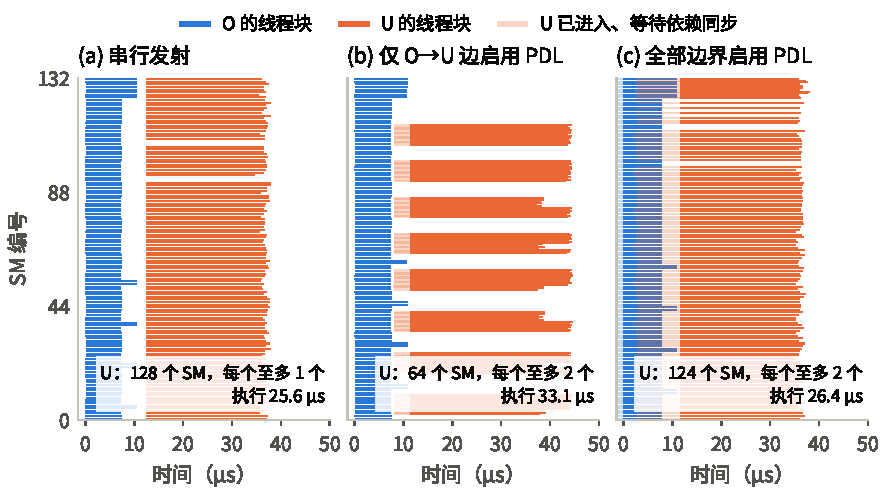
\includegraphics[width=\textwidth]{Img/midterm/v4_timeline}
\caption{真实模型 prefill 1$\times$16（第 2 层）中 O$\to$U 边界在三种模式下的 SM 执行时间线。每条水平线段对应一个线程块的执行起止区间：(a) 串行发射下 U 均匀分布；(b) 仅该边启用 PDL 时 U 因档位不兼容集中落入先空闲的少数 SM；(c) 全链启用 PDL 时 SM 维持高档位，U 恢复提前并发执行且分布均衡。}\label{fig:timeline}
\end{figure}

基于设备端时间戳归纳出的分批均衡派发模型（按约 0.9\us 周期扫描满足档位与余量的候选 SM 并均匀派发待命块），仅利用纯串行运行中记录的前驱退出时刻即可预测 PDL 后继线程块的 SM 分配结果：如表~\ref{tab:place} 所示，在 442 次样本外跨边界发射上，最拥挤 SM 块数的精确命中率达 90\%（两类不可共驻边界分别为 146/146 与 120/124）。受控探针实验（图~\ref{fig:pack}）进一步证实，单 SM 挤入 3 块时实际获取的访存带宽仅为单块 SM 的 1.7 倍，负载不均将尾时延拉长 5.3--7.2\us，与真实模型 7.6\us 的性能退化吻合。

\begin{table}[!htb]\centering
\caption{分批派发模型对 PDL 后继线程块 SM 分配结果的预测精度。命中定义为最拥挤 SM 上的预测后继块数与实测完全一致；SM 数误差给出占用 SM 数绝对偏差的中位数与 90 分位数}\label{tab:place}
\footnotesize\setlength{\tabcolsep}{3.8pt}
\begin{tabular}{@{}lcccccc@{}}
\toprule
 & \multicolumn{3}{c}{基于同次运行退出时刻复现} & \multicolumn{3}{c}{基于串行运行退出时刻样本外预测}\\
\cmidrule(lr){2-4}\cmidrule(l){5-7}
物理边界类别 & 发射次数 & 精确命中 & SM 数误差 & 发射次数 & 精确命中 & SM 数误差\\
\midrule
可提前共驻 SM & 368 & 222（60\%） & 0 / 16 & 172 & 134（78\%） & 0 / 4 \\
不可共驻、后继占满全卡 & 286 & 286（100\%） & 0 / 0 & 146 & 146（100\%） & 0 / 0 \\
不可共驻、后继未占满全卡 & 236 & 225（95\%） & 3 / 44 & 124 & 120（97\%） & 2 / 10 \\
\bottomrule
\end{tabular}
\end{table}

\begin{figure}[!htb]\centering
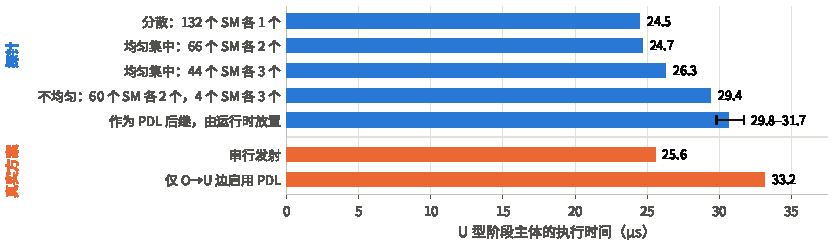
\includegraphics[width=0.94\textwidth]{Img/midterm/v4_pack}
\caption{不同跨 SM 线程块分布对后继执行时间的影响。上图为 U 型矩阵探针（128$\times$16 分块，132 块）在五种空间分布下的耗时，集中调度及真实 PDL 分配显著拉长尾时延；下图对照真实模型 U 阶段在串行与单边 PDL 下的耗时。}\label{fig:pack}
\end{figure}

\subsubsection{L1 缓存容量缩水分析与静态 PDL 启用规则}\label{sec:edge}\label{sec:answer}

除 SM 负载不均外，上述“SM 档位沿执行链保持”的硬件规则还会引发第二类性能退化：\textbf{低共享内存需求的后继如果提前进入高档位前驱 SM，会沿用前驱的大共享内存配置，导致可用的 L1 缓存容量缩水}（图~\ref{fig:carve}(c)）。为了单独量化这一效应，我们在纯串行发射下强制全图采用最大 228\,KiB 共享内存档位进行对照测试（图~\ref{fig:lone}）：显式使用共享内存双缓冲的矩阵阶段几乎不受 L1 容量影响（九成变化在 $\pm 1.4\%$ 以内）；但高度依赖 L1 缓存复用键值数据的 prefill Flash\allowbreak{}Attention-2 变慢 7.3\%--15.5\%，长序列逐 warp attention（$1\times 256$）耗时更由 117\us 飙升至 191\us（增幅 63\%），与全链开启 PDL 时的实测减速一一对应（图~\ref{fig:lone}(b)）。

\begin{figure}[!htb]\centering
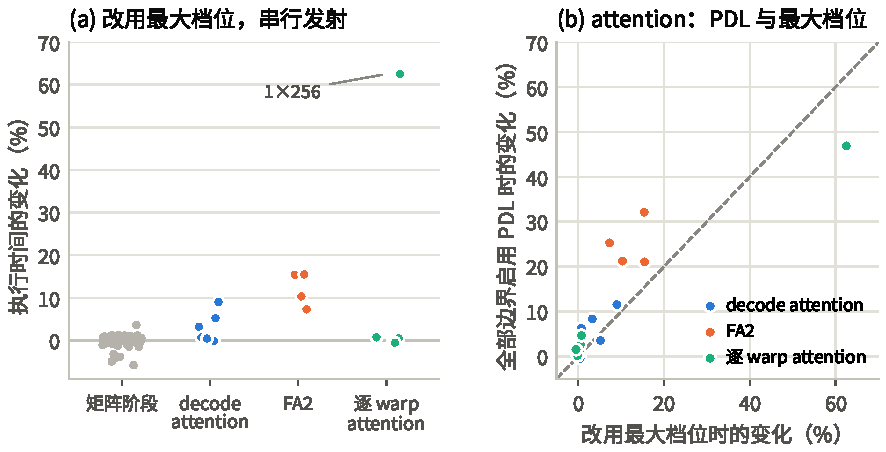
\includegraphics[width=\textwidth]{Img/midterm/v4_l1}
\caption{算子阶段对共享内存 carve-out 档位（剩余 L1 容量）的敏感度差异及其对 PDL 减速的解释。(a) 纯串行发射下强制最大档位引发的各阶段耗时变化；(b) 全链启用 PDL 时 attention 的实际减速幅度与离线测得的 L1 敏感度高度吻合。}\label{fig:lone}
\end{figure}

综合“SM 负载不均”与“L1 缓存缩水”两项硬件机理，仅凭编译期已知的寄存器数、动态共享内存、启动线程块数及对应 carve-out 档位，就可以将任意物理边界静态归入三类：（1）可提前共驻 SM；（2）不可提前共驻但后继线程块占满全卡；（3）不可提前共驻且后继未占满全卡。如图~\ref{fig:cmpdl} 与表~\ref{tab:cmrule} 在 253 类实测物理边界上的检验所示：后继以矩阵阶段开头时，前两类的 113 类边界中有 106 类（94\%）加速、0 类减速（中位数 $+1.0$\us/边），而第三类中有 58\% 减速（最差 $-9.8$\us/边）。由此导出\textbf{基于编译期信息的静态 PDL 启用规则}：
\begin{quote}\small
一条物理边界启用 PDL，当且仅当沿执行链当前生效档位判定该边属于“可提前共驻 SM”或“后继占满全卡”，且若后继以 attention 开头并将沿用更高档位时，其离线测得的 L1 容量缩水代价不超过单次边界节省量（1.0\us）。
\end{quote}
阶段图相邻算子边的完整处理规则汇总于表~\ref{tab:answer}。

\begin{figure}[!htb]\centering
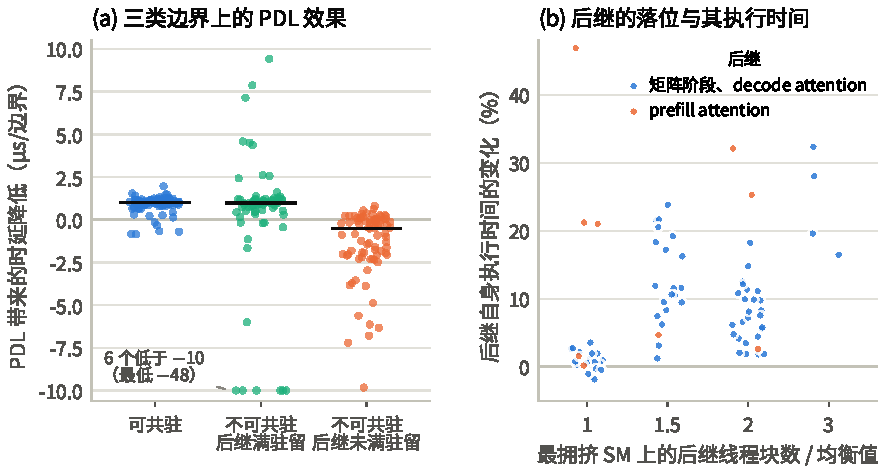
\includegraphics[width=\textwidth]{Img/midterm/v3_pdl}
\caption{物理边界静态三分类对 PDL 实测净收益的区分能力。(a) 253 类边界按静态资源特征分为三类后的单边时延变化分布（横线为中位数）；(b) 16 个全切分方案中后继最拥挤 SM 块数集中程度与后继执行时间增幅的对应关系。}\label{fig:cmpdl}
\end{figure}

\begin{table}[!htb]\centering
\caption{静态三分类在 253 类实测物理边界上的 PDL 单边收益统计（\textmu s/边界，正值表示加速，按后继首阶段类型分列）}\label{tab:cmrule}
\footnotesize\setlength{\tabcolsep}{3.8pt}
\begin{tabular}{@{}llccccccc@{}}
\toprule
静态边界类别 & 后继首阶段 & 样本数 & 中位数 & 四分位区间 & 最差值 & 加速 & 持平 & 减速\\
\midrule
可提前共驻 SM & 矩阵阶段 & 80 & $+1.04$ & $+0.95$ 至 $+1.15$ & $+0.6$ & 80 & 0 & 0 \\
 & Attention & 22 & $+0.58$ & $-0.16$ 至 $+0.89$ & $-0.9$ & 15 & 2 & 5 \\
不可共驻、后继占满全卡 & 矩阵阶段 & 33 & $+1.12$ & $+0.95$ 至 $+2.43$ & $-1.7$ & 26 & 7 & 0 \\
 & Attention & 37 & $+0.69$ & $-0.17$ 至 $+1.07$ & $-47.6$ & 25 & 5 & 7 \\
不可共驻、后继未占满全卡 & 矩阵阶段 & 71 & $-0.89$ & $-2.20$ 至 $+0.03$ & $-9.8$ & 10 & 20 & 41 \\
 & Attention & 10 & $-0.39$ & $-0.80$ 至 $-0.00$ & $-1.4$ & 2 & 1 & 7 \\
\bottomrule
\end{tabular}
\end{table}

\begin{table}[!htb]\centering
\caption{阶段依赖图相邻算子边的处理规则与依据汇总}\label{tab:answer}
\small
\begin{tabularx}{\textwidth}{@{}>{\raggedright\arraybackslash}X>{\raggedright\arraybackslash}p{3.7cm}>{\raggedright\arraybackslash}p{3.2cm}@{}}
\toprule
边界两侧阶段的资源与调度特征 & 选定边处理方式 & 支撑依据\\
\midrule
两侧资源需求接近，融合执行无额外损失（如单请求短上下文 decode、极短序列逐 warp prefill） & 保留同 grid 融合（配合核内分阶段活跃块控制） & 表~\ref{tab:cores}，表~\ref{tab:decode}\\
一侧需更高线程块并发、占满寄存器预算或偏好不同分块，融合资源损失高于单次启动开销 & 切分为物理边界，两侧分组独立配置分块与块数 & 表~\ref{tab:cores}，图~\ref{fig:rule}\\
已切分物理边界；后继可提前共驻 SM 或已占满全卡，且无超阈值 L1 缩水代价 & 启用跨 grid PDL（后继含静态权重且有带宽余量时可预载 1\,MiB） & 表~\ref{tab:cmrule}，图~\ref{fig:rulereal}\\
已切分物理边界；后继不可提前共驻且未占满全卡（易引发先空闲 SM 上的集中调度） & 采用跨 grid completion 串行执行 & 图~\ref{fig:timeline}，表~\ref{tab:cmrule}\\
已切分物理边界；后继为 L1 敏感的 attention 且提前进入将沿用高档位 & 采用跨 grid completion 串行执行 & 图~\ref{fig:lone}，图~\ref{fig:rulereal}\\
\bottomrule
\end{tabularx}
\end{table}

\subsection{划分方案搜索与动态 Shape 自适应框架}\label{sec:search_sys}\label{sec:sys}

有了执行机制和静态 PDL 规则后，本节回答问题四：面临庞大的分组切分与参数配置组合，如何在不逐点真机穷举的前提下快速构造高质量划分方案？当线上请求 batch 与序列长度动态变化时，又该如何低开销地切换执行计划？

\subsubsection{基于线程块波次的分组耗时解析模型}\label{sec:cm}

要避免每次改变输入规模都在真机上遍历上百组配置，核心在于建立足够准确、又能跨配置泛化的分组耗时解析模型。我们自底向上拆解矩阵与 attention 阶段的执行耗时：

在\textbf{矩阵主循环层面}，权重常驻 L2 时的部件消融实验（图~\ref{fig:ablate}）表明，小分块主循环主要受片上异步装载通路限制：$128\times 16$ 与 $64\times 64$ 分块剥离异步拷贝可缩短每步耗时 28\%--41\%，明显大于剥离 MMA 计算指令的 18\%--26\%；每 SM 并发 3 块时，纯异步拷贝甚至因装载通路饱和而反慢于完整循环。当权重需从 HBM 流式读取时（图~\ref{fig:cmloop}），每步耗时随并发读取的相异权重块数迅速触及 2.96\,TB/s 带宽上限，随输入行数 $M$ 增大则借助行方向权重复用平滑过渡到计算主循环受限。

\begin{figure}[!htb]\centering
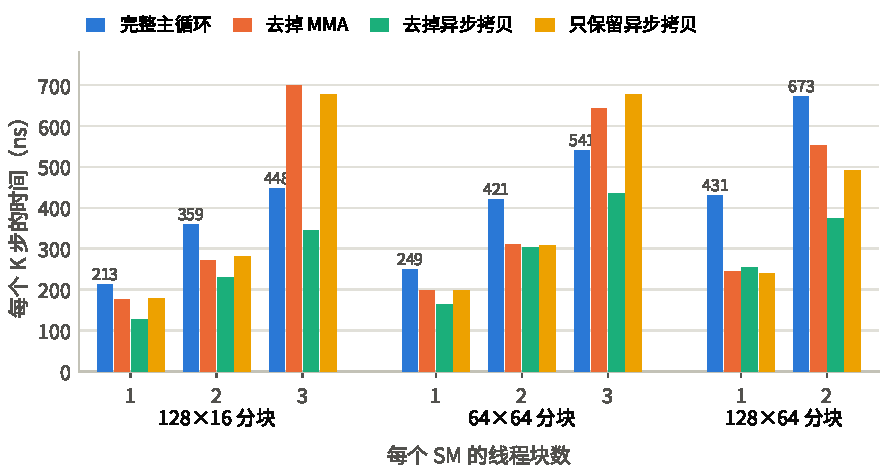
\includegraphics[width=0.95\textwidth]{Img/midterm/v4_ablate}
\caption{矩阵主循环部件消融实验（权重常驻 L2 时单个 K 步耗时）。小分块下剥离异步拷贝节省的时间显著高于剥离 MMA 指令；每 SM 并发 3 块时纯异步拷贝因装载通路过载反慢于完整循环。}\label{fig:ablate}
\end{figure}

\begin{figure}[!htb]\centering
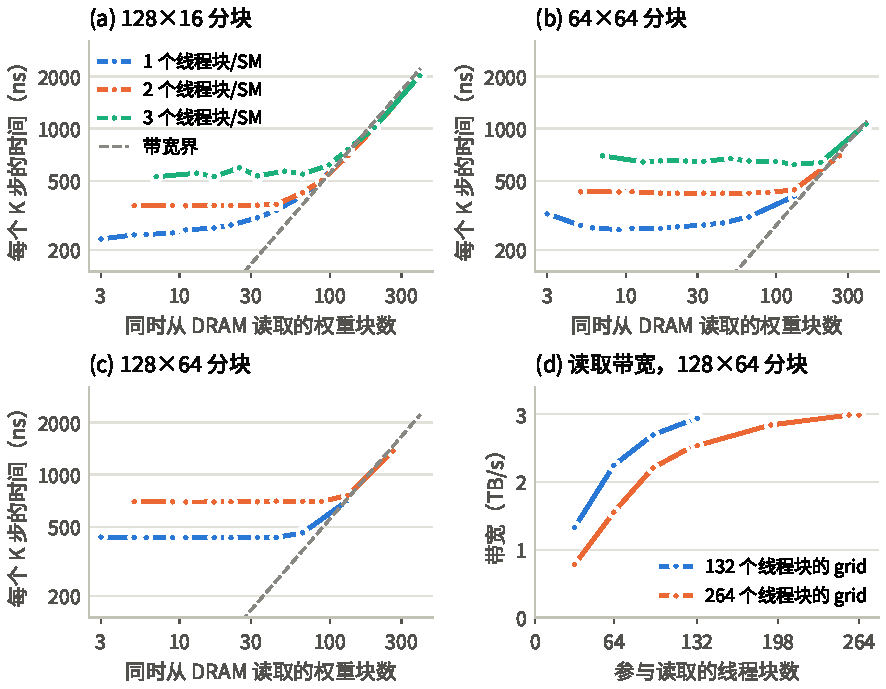
\includegraphics[width=0.94\textwidth]{Img/midterm/v3_loop}
\caption{片外流式读取下每个 K 步耗时向 HBM 带宽上限的过渡规律。(a)--(c) 三种分块形状下每步耗时随并发读取相异权重块数的变化（虚线为 2.96\,TB/s 带宽界）；(d) 128$\times$64 分块下有效读取带宽随参与线程块数的变化。}\label{fig:cmloop}
\end{figure}

在\textbf{完整单阶段层面}，扫描 1 至 2048 行的 43 个行数（共 1376 个测点）可以清晰看到由线程块波次（wave quantization）主导的阶梯曲线（图~\ref{fig:cmladder}）：每当行数越过分块行数整数倍导致总波数 $W$ 加一，耗时就会阶跃上升（如 U 阶段从 128 行的 32.0\us 跨入 129 行第二波时跃升至 47.0\us，增幅 47\%）。结合核内计时分解（表~\ref{tab:cmtl}），矩阵阶段总耗时可解析表达为固定开销、多波主循环与尾部逐元素第二遍三项之和：
\begin{equation}
T=T_{\mathrm{fix}}+\sum_{w=1}^{W}\bigl[t_{\mathrm{wave}}(n_w,c_w,k)+t_{\mathrm{epi}}\bigr]+T_{\mathrm{2nd}}, \label{eq:stage}
\end{equation}
其中波数 $W$、第 $w$ 波新读权重块数 $n_w$、单 SM 参与块数 $c_w$ 与单任务 K 步数 $k$ 均由分块映射直接算得；完全复用微探针常数而不实测真实阶段的为模型 A（留出中位误差 3.9\%），仅在 16、64、2048 三个采样行数标定尾部系数的为模型 B（留出中位误差 3.4\%）。

\begin{figure}[!htb]\centering
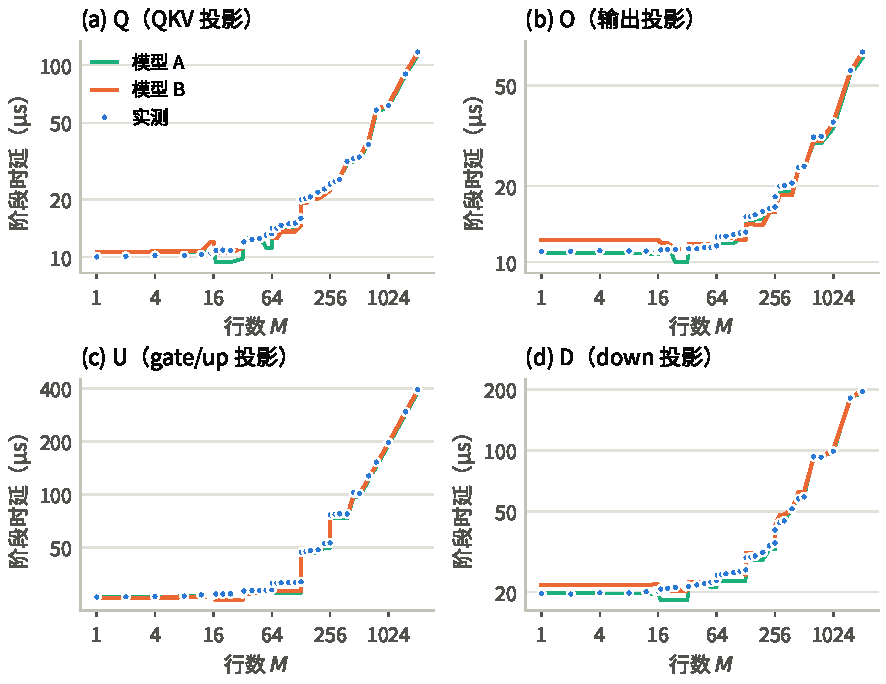
\includegraphics[width=\textwidth]{Img/midterm/v3_ladder}
\caption{四个矩阵阶段独立成组时随输入行数的波次阶梯曲线及解析模型拟合效果。模型 A 完全复用微探针常数，模型 B 仅使用 16、64 与 2048 三个采样行数标定尾部系数，均准确复现了其余 40 个留出行数上的台阶位置与幅值。}\label{fig:cmladder}
\end{figure}

\begin{table}[!htb]\centering
\caption{矩阵阶段独立成组时核内各组成部分的实测耗时分解（\textmu s，取对应行数最优分块/块数配置）}\label{tab:cmtl}
\footnotesize\setlength{\tabcolsep}{4.2pt}
\begin{tabular}{@{}lrlccrrrrrr@{}}
\toprule
阶段 & 行数 & 最优配置 & \makecell{K 维\\切分} & 波数 & \makecell[r]{固定\\开销} & \makecell[r]{主循\\环遍} & \makecell[r]{核内\\屏障} & \makecell[r]{尾部第\\二遍} & 计时合计 & 生产实测\\
\midrule
Q & 16 & 128$\times$16 / 264 & 8 & 1 & 2.2 & 6.6 & 1.2 & 1.0 & 11.0 & 10.8 \\
Q & 256 & 64$\times$64 / 396 & 2 & 1 & 2.3 & 13.3 & 1.5 & 6.0 & 23.2 & 23.6 \\
Q & 2048 & 128$\times$64 / 264 & 1 & 3 & 2.3 & 71.2 & 1.2 & 40.8 & 115.6 & 116.9 \\
O & 16 & 128$\times$16 / 132 & 8 & 1 & 2.1 & 4.7 & 1.2 & 3.5 & 11.7 & 11.2 \\
O & 256 & 64$\times$64 / 264 & 2 & 1 & 2.2 & 9.1 & 1.7 & 3.1 & 16.3 & 16.5 \\
O & 2048 & 128$\times$64 / 264 & 1 & 2 & 2.2 & 49.9 & 1.1 & 14.5 & 67.8 & 67.9 \\
U & 16 & 128$\times$16 / 132 & 1 & 1 & 2.3 & 24.3 & -- & -- & 26.8 & 27.0 \\
U & 256 & 128$\times$64 / 264 & 1 & 2 & 2.2 & 50.6 & -- & -- & 53.0 & 53.1 \\
U & 2048 & 128$\times$64 / 264 & 1 & 16 & 2.2 & 388.7 & -- & -- & 391.0 & 394.1 \\
D & 16 & 128$\times$16 / 132 & 8 & 1 & 2.2 & 12.8 & 1.2 & 3.8 & 20.1 & 20.3 \\
D & 256 & 128$\times$64 / 264 & 4 & 1 & 2.2 & 26.8 & 1.3 & 4.2 & 34.7 & 35.0 \\
D & 2048 & 128$\times$64 / 264 & 1 & 2 & 2.2 & 180.1 & 1.1 & 16.3 & 199.7 & 195.9 \\
\bottomrule
\end{tabular}
\end{table}

进一步发现，当每 SM 并发 3 个线程块时，同 SM 内三个线程块之间稳定存在 17\% 的速度差异（14.6\us 至 17.1\us），而整波完成时间由最慢的那一块决定。将单波时长 $t_{\mathrm{wave}}$ 由中位数修正为同 SM 最慢线程块耗时后，模型 A 在每 SM 3 块下的留出中位误差由 10.9\% 降至 3.8\%（图~\ref{fig:order}，模型 B 为 3.5\%）。连同按最重工作单元建立的三种 attention 参数化模型，单阶段留出集精度汇总于表~\ref{tab:cm_all_acc}（矩阵阶段仅实测模型推荐的前 2 个配置即可将相对最优的平均性能损失压至 0.34\%）。

在\textbf{多阶段融合分组层面}，任意连续多阶段分组 $g$ 的耗时无需新增组合拟合参数，直接由固定开销、各阶段主体耗时与核内屏障线性相加得到：
\begin{equation}
T_g=T_{\mathrm{fix}}+\sum_{s\in g}B_s(x,\theta_g)+(|g|-1)\,t_{\mathrm{bar}}. \label{eq:group}
\end{equation}
在真实模型采集的全部 2177 组配置上检验（图~\ref{fig:group} 与表~\ref{tab:group}），整体中位误差仅为 4.9\%，其中纯矩阵多阶段分组误差（2.9\%--3.5\%）与单阶段基本持平；仅含高寄存器 FlashAttention-2 的融合分组因跨阶段指令相互干扰误差偏高（15.3\%），将作为下一阶段模型精细化的重点。

\begin{figure}[!htb]\centering
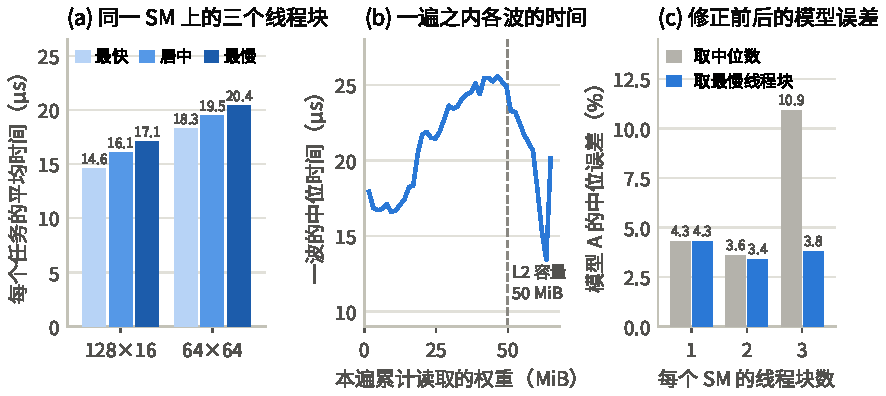
\includegraphics[width=0.95\textwidth]{Img/midterm/v4_order}
\caption{高并发密度下同 SM 线程块的速度差异及其对模型精度的修正效果。(a) 每 SM 并发 3 块时同 SM 内快、中、慢三个线程块的单任务耗时差异；(b) 多波推进过程中随累计权重逼近 L2 容量出现的单波耗时抬升；(c) 改按最慢线程块建模前后在三种并发密度下的留出集中位误差对比。}\label{fig:order}
\end{figure}

\begin{table}[!htb]\centering
\caption{单阶段解析模型（模型 B）在留出测试集上的时延预测误差与配置选择精度}\label{tab:cm_all_acc}
\footnotesize\setlength{\tabcolsep}{4.2pt}
\begin{tabular}{@{}llccccc@{}}
\toprule
阶段类型 & 评估对象 & \makecell{检验\\测点数} & \makecell{中位误\\差（\%）} & \makecell{90 分位\\误差（\%）} & \makecell{命中实测\\最优比例} & \makecell{相对最优平\\均损失（\%）}\\
\midrule
矩阵阶段 & Q 阶段 & 320 & 3.2 & 8.9 & \multirow{4}{*}{140/160（Top-2）} & \multirow{4}{*}{0.34（Top-1: 1.39）} \\
 & O 阶段 & 320 & 4.1 & 10.7 &  &  \\
 & U 阶段 & 320 & 3.4 & 10.7 &  &  \\
 & D 阶段 & 320 & 2.9 & 8.1 &  &  \\
 & 四阶段汇总 & 1280 & 3.4 & 10.0 & 140/160 & 0.34 \\
\midrule
Attention & Decode 切片归约 & 100 & 5.1 & 15.8 & 14/25（Top-1） & 3.70 \\
 & Prefill，FA2 & 28 & 6.5 & 19.8 & 14/14（Top-1） & 0.00 \\
 & Prefill，逐 warp & 56 & 12.1 & 21.2 & 13/14（Top-1） & 0.10 \\
\bottomrule
\end{tabular}
\end{table}

\begin{figure}[!htb]\centering
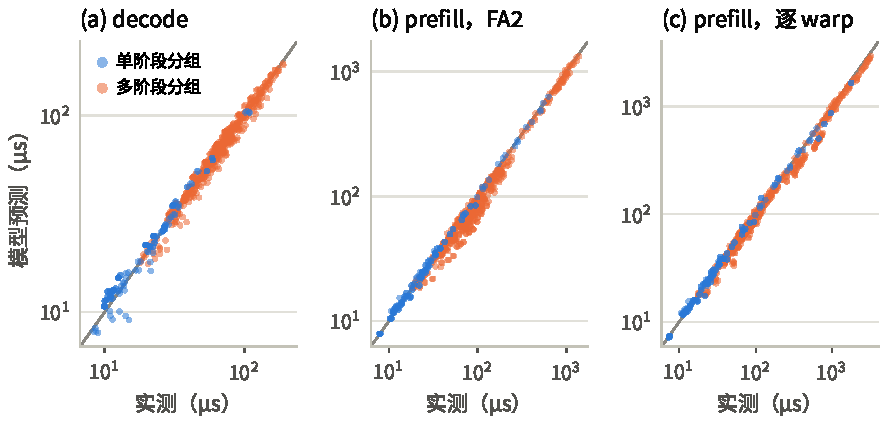
\includegraphics[width=0.94\textwidth]{Img/midterm/v3_group}
\caption{零组合拟合参数下多阶段分组模型预测值与真实模型 2177 组实测耗时的对比散点图（不含首尾词嵌入与词表投影分组）。}\label{fig:group}
\end{figure}

\begin{table}[!htb]\centering
\caption{分组时延模型在 2177 组真实模型配置上的相对误差分布（\%，报告中位数与 90 分位数）}\label{tab:group}
\footnotesize\setlength{\tabcolsep}{4.5pt}
\begin{tabular}{@{}lccccccccc@{}}
\toprule
 & & \multicolumn{2}{c}{全部配置} & \multicolumn{2}{c}{单阶段分组} & \multicolumn{2}{c}{\makecell{多阶段分组\\（不含 attention）}} & \multicolumn{2}{c}{\makecell{多阶段分组\\（含 attention）}}\\
\cmidrule(lr){3-4}\cmidrule(lr){5-6}\cmidrule(lr){7-8}\cmidrule(l){9-10}
阶段与实现 & 配置总数 & 中位 & 90 分位 & 中位 & 90 分位 & 中位 & 90 分位 & 中位 & 90 分位\\
\midrule
Decode & 731 & 4.1 & 12.7 & 7.8 & 16.0 & 3.5 & 11.8 & 4.0 & 11.5 \\
Prefill，FA2 & 672 & 5.8 & 23.7 & 2.7 & 9.4 & 2.9 & 9.0 & 15.3 & 30.7 \\
Prefill，逐 warp & 774 & 5.2 & 16.3 & 3.3 & 10.9 & 3.0 & 8.9 & 8.0 & 23.5 \\
\bottomrule
\end{tabular}
\end{table}

\subsubsection{模型与静态规则引导的离线规划方法}\label{sec:search}\label{sec:guided}

在没有代价模型和静态规则辅助时，基准穷举规划器需要在每个输入规模上遍历全部多阶段分组配置、端到端实测全部 32 种切分方案并逐边贪心搜索 PDL 开关，单负载耗时达 35--262\,s。结合式~(\ref{eq:group}) 的分组耗时模型与第~\ref{sec:edge}~节的静态 PDL 启用规则，课题将其压缩为紧凑的\textbf{四步引导式离线规划流程}：
\begin{enumerate}[leftmargin=2.4em,itemsep=2pt]
\item \textbf{分组配置筛选}：对不含首尾层的多阶段分组直接按式~(\ref{eq:group}) 排序并仅实测排名第一的配置；单阶段分组扫描基准块数，并为 attention 加测一次最大共享内存档位以标定其 L1 缩水代价；
\item \textbf{切分拓扑粗排}：以各分组最优耗时之和减去静态规则核准的 PDL 预计节省量（按 1.0\us/边计）为 31 种切分方案快速打分，仅截取前 6 名进入端到端实测候选；
\item \textbf{PDL 规则生成}：取消逐边贪心试探，直接为入围切分方案生成静态规则集合、附带 1\,MiB 权重预载集合、链式档位一致集合与全开对照（每拓扑至多 4 个变体）；
\item \textbf{端到端定案}：在选择集上将上述候选与最优单一 grid 实测对比，输出最终计划。
\end{enumerate}
该流程在几乎不损失端到端性能的前提下将真机测量量大幅削减（具体评测见第~\ref{sec:exp}~节）。

\subsubsection{动态 Shape 决策分类与离线—在线协同架构}\label{sec:types}\label{sec:arch}

要处理线上推理中 batch 和序列长度的动态变化，不可能在每次前向推理时重新运行规划器，必须搞清楚执行计划 $\Pi=\langle C,\{\theta_g\},\{\varphi_e\}\rangle$ 中哪些决策可以离线写死、哪些必须随输入规模调整。为此，我们在 15 个代表负载上全量采集了单一 grid 与 31 种切分方案（累计 1649 个端到端方案）的交替重放时延，以“将某项决策固定后，在全部负载上最多会慢多少”为衡量标准，在 1.0\% 容差内将执行计划划分为三类：
\begin{enumerate}[leftmargin=2.4em,itemsep=2pt]
\item \textbf{固定型决策（离线固化）。}如图~\ref{fig:types}(a) 所示，同属矩阵阶段、资源需求一致的 U$\to$D 边在全部负载上固定融合的最大损失不超过 0.3\%；decode 阶段其余四条边统一固定为切分（即 Q|A|O|UD 分组）跨全负载最大损失也仅 0.6\%。
\item \textbf{切换型决策（仅保留两种机制候选）。}prefill 阶段除 U$\to$D 外的四条边随融合代价由负转正同步切换（图~\ref{fig:types}(b)）。因此切分层无需保留全部 32 种拓扑，只保留\textbf{“全模型单一 grid”和“Q|A|O|UD 四边切分”两个候选}（图~\ref{fig:types}(c)），即可将跨负载切分损失压在 0.6\% 以内（无先验自动选两项也仅 1.4\%）；而各物理边界的 PDL 开关由静态规则直接导出，在 Q|A|O|UD 上相对串行稳定提速 0.8\%--4.2\%。
\item \textbf{参数型决策（按有效行数分区间建表）。}与切分方式高度收敛相反，各分组的分块形状与线程块数随输入行数高频变化（图~\ref{fig:tile}）：43 个扫描行数上四个矩阵阶段经历 5--16 次切换，固定单一配置的最大损失高达 16\%--22\%（decode attention 固定 528 块最大损失达 26\%）。不过，在 1\% 容差内合并相邻最优配置相同的行数后，覆盖全部行数只需约 22 个有效行数区间（5\% 容差下缩至 15 个区间）。
\end{enumerate}

\begin{figure}[!htb]\centering
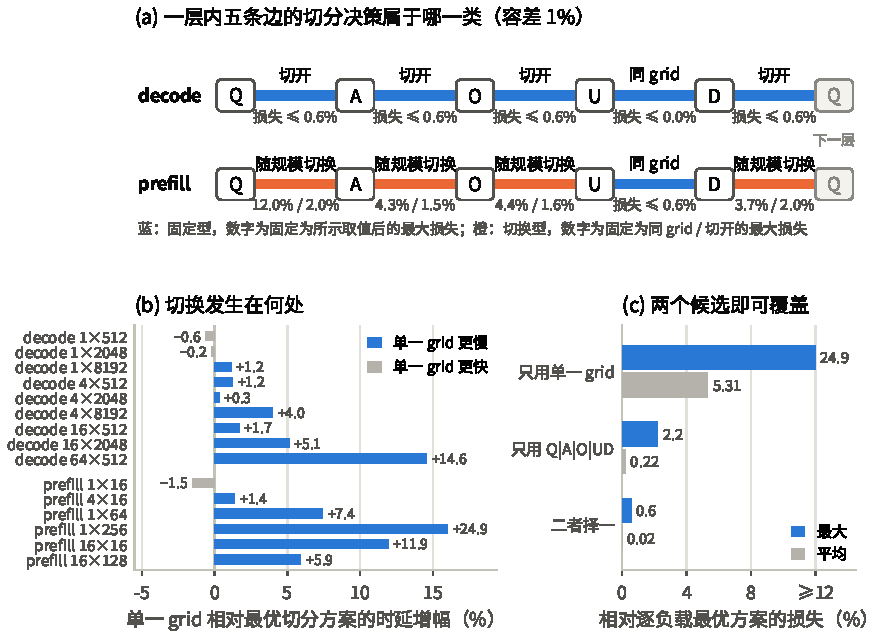
\includegraphics[width=\textwidth]{Img/midterm/v5_colour}
\caption{容差 1\% 下五类算子边切分决策的敏感度分类与候选压缩效果。(a) Decode 与 prefill 阶段各边切分决策所属类别及固定后的最大相对时延损失；(b) 各负载下单一 grid 相对最优切分方案的时延增幅；(c) 切分层仅保留单一候选或双候选集合时的跨负载最大与平均损失。}\label{fig:types}
\end{figure}

\begin{figure}[!htb]\centering
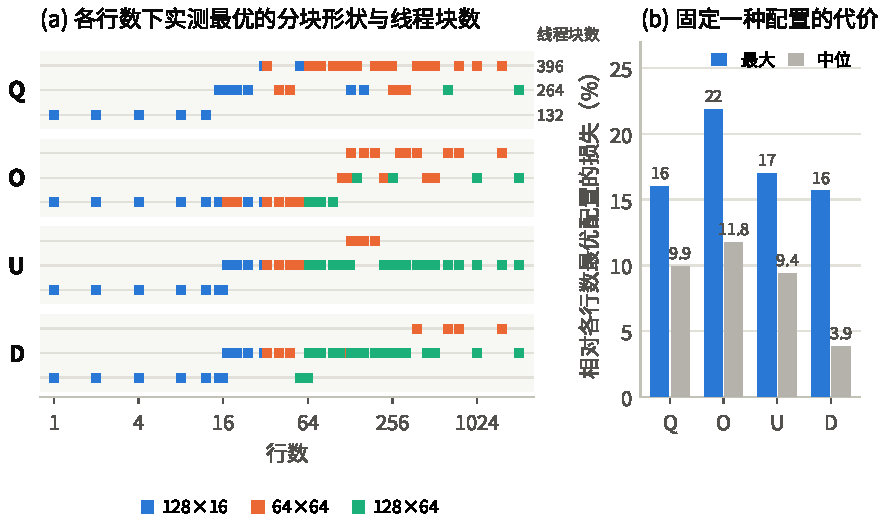
\includegraphics[width=\textwidth]{Img/midterm/v5_tile}
\caption{分组资源配置沿输入行数轴的参数型跳变特征。(a) 四个矩阵阶段在 43 个行数上实测最优的分块形状与启动线程块数；(b) 全局固定采用单一配置（128$\times$64 分块、264 个线程块）相对逐行数最优配置的时延损失。}\label{fig:tile}
\end{figure}

基于上述三类划分，课题确立了如图~\ref{fig:arch} 所示的\textbf{“离线准备—在线选择”两阶段系统架构}：离线阶段（每个模型与目标 GPU 只执行一次）完成统一后端编译、模型与静态规则引导规划、决策分类，并按有效行数区间组织双候选执行方案、分组资源配置及预捕获 CUDA Graph 候选计划表；在线阶段（每次前向推理）根据实时请求的 batch 和序列长度算出有效行数，查表取出对应计划并更新运行参数直接重放，保证候选表规模线性可控且在线路径零搜索。目前离线侧候选生成、引导规划与 15 负载决策分类已完成，二维全网格计划表与在线查表执行器将在下一阶段（2027.01–04）落地实现。

\begin{figure}[!htb]\centering
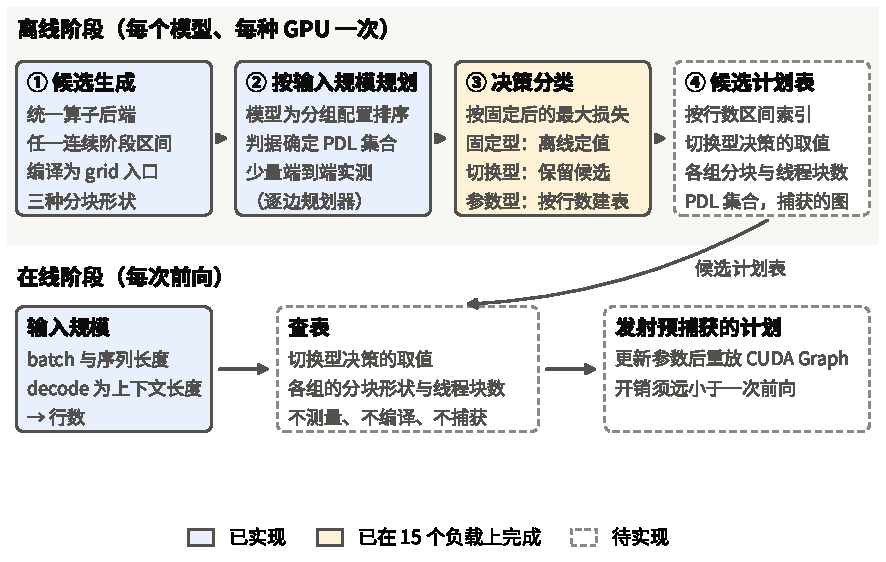
\includegraphics[width=\textwidth]{Img/midterm/v5_arch}
\caption{面向动态输入规模的“离线准备—在线选择”两阶段系统架构。离线阶段一次性完成统一算子编译、模型与规则引导规划、规模敏感度分类及候选计划表构建；在线阶段根据实时请求有效行数直接查表重放预捕获 CUDA Graph。}\label{fig:arch}
\end{figure}

\subsection{阶段性实验评估与分析}\label{sec:exp}

本节在真实模型权重与英文文本语料上，依次评估上述自适应执行机制的端到端性能收益、静态 PDL 规则的可靠性以及模型引导规划器的搜索效率。

\subsubsection{实验环境与评测设置}

全部实验在单张 NVIDIA H100 80GB HBM3 GPU（132 个 SM，CUDA 12.3）上基于 Llama-3.2-1B-Instruct 的 BF16 权重执行，覆盖 9 组 decode 负载（batch $\times$ 缓存上下文长度）与 6 组 prefill 负载（batch $\times$ 输入序列长度）。真实语料严格切分为互不重叠的选择集与报告集：规划搜索仅使用选择集，最终时延与 95\% 分块自助法置信区间均在报告集上经 CUDA Graph 捕获后通过 20 个随机乱序测量块交替重放获取。所有参评方案均通过严格数值正确性检查：贪心采样输出与 Hugging Face 参考实现完全一致，logits KL 散度不超过 0.02，新写入 KV 缓存相对二范数误差不超过 4\%。对比基线分为四类：（1）全阶段统一线程块数的“统一配置单一 grid”；（2）加入逻辑块重排与核内分阶段活跃块控制的“最优单一 grid”；（3）固定全切分串行与全局开启 PDL 方案；（4）主流外部推理系统 vLLM~\pVllm 与 Mirage MPK~\pMPK。

\subsubsection{端到端性能收益与对比分析}

表~\ref{tab:decode} 与表~\ref{tab:prefill} 汇总了 15 个基准负载上的端到端评测结果，图~\ref{fig:gain} 展示了不同机制对端到端加速的逐层贡献：
\begin{itemize}[leftmargin=2.0em,itemsep=2pt]
\item \textbf{Decode 阶段（表~\ref{tab:decode}）：}规划器在 8 个负载上选出含物理切分与逐边 PDL 的方案（主要收敛至 Q|A|O|UD 与全切分，仅 $1\times 2048$ 保留单一 grid），相对最优单一 grid 缩短单步时延 0--13.0\%（相对统一配置单一 grid 缩短 0.1\%--13.0\%）。按贡献来源拆解（图~\ref{fig:gain}(a)）：核内分阶段活跃块控制先为单核基线消除最高 6.0\% 内部并发失配；物理切分使 attention 突破 396 块上限扩展至 528 块，在 $4\times 8192$、$16\times 2048$ 与 $64\times 512$ 上直接贡献最高 11.6\% 降幅；逐边 PDL 进一步削减 1.6\%--5.4\% 算子间等待间隙，使原本单纯切分变慢的中小批量负载（$1\times 8192$、$4\times 512$、$16\times 512$）转为正收益。相比之下，固定全切分串行（$-5.4\%$ 至 $+10.4\%$）与全局开启 PDL（$-1.7\%$ 至 $+7.1\%$）均在多个工作点性能退化。
\item \textbf{Prefill 阶段（表~\ref{tab:prefill}）：}相对取较快 attention 实现的最强单一 grid 基线，规划方案缩短首 token 时延 0--19.2\%（图~\ref{fig:gain}(b)）。序列长度 16 的单请求负载由逐 warp 单核即达最优（1352.5\us），而 $16\times 16$ 因矩阵与 attention 偏好不同配置仍获 9.61\% 降幅；序列长度增至 64 及以上后，物理切分将占满 255 寄存器的 FlashAttention-2 隔离至独立 kernel，使相邻矩阵分组恢复每 SM 3 块并发，在 $1\times 64$、$1\times 256$ 与 $16\times 128$ 上分别取得 8.43\%、19.23\% 与 5.21\% 加速。
\item \textbf{收益规律与外部系统对比：}将 15 个负载的端到端收益与 16 层累计共驻代价占比对照（图~\ref{fig:rule}），二者 Spearman 秩相关系数达 $\rho=0.92$：累计共驻代价占比超 8\% 的 7 个负载仅凭切分即获超 4.5\% 加速；其余 8 个低代价负载中，6 个靠逐边 PDL 获 0.2\%--1.95\% 正收益，2 个自动保留单一 grid。横向对比主流外部系统，规划方案在全部 decode 与中小规模 prefill 负载上较 vLLM~\pVllm 分别缩短时延 25\%--41\% 与 41\%--71\%，在单请求负载（decode $1\times 512$、prefill $1\times 16$ 与 $1\times 64$）上较 Mirage MPK~\pMPK 分别提速 21\%、33\% 与 79\%。
\end{itemize}

\begin{table}[!htb]\centering
\caption{Decode 阶段端到端单步时延（\textmu s）及规划方案相对两级单一 grid 基线的时延降幅（\%）}\label{tab:decode}
\small
\begin{tabular}{@{}lrrrrr@{}}
\toprule
测试负载 & \makecell[r]{统一配置\\单一 grid} & \makecell[r]{最优\\单一 grid} & 规划方案 & \makecell[r]{相对统一配置\\降幅（\%）} & \makecell[r]{相对最优单一 grid 降幅\\及 95\% 置信区间（\%）}\\
\midrule
1$\times$512 & 1368.5 & 1366.8 & 1364.1 & $+0.3$ & $+0.19$ [0.17, 0.24] \\
1$\times$2048 & 1439.5 & 1438.0 & 1438.0 & $+0.1$ & 0 \\
1$\times$8192 & 1640.4 & 1628.8 & 1597.1 & $+2.6$ & $+1.95$ [1.54, 2.09] \\
4$\times$512 & 1428.7 & 1428.2 & 1405.1 & $+1.7$ & $+1.62$ [1.34, 1.74] \\
4$\times$2048 & 1604.3 & 1562.5 & 1545.7 & $+3.6$ & $+1.07$ [1.02, 1.12] \\
4$\times$8192 & 2137.9 & 2030.3 & 1938.8 & $+9.3$ & $+4.50$ [4.43, 4.58] \\
16$\times$512 & 1681.8 & 1616.4 & 1592.4 & $+5.3$ & $+1.49$ [1.34, 1.64] \\
16$\times$2048 & 2201.8 & 2070.8 & 1974.4 & $+10.3$ & $+4.65$ [4.52, 4.79] \\
64$\times$512 & 2514.6 & 2514.4 & 2187.0 & $+13.0$ & $+13.02$ [12.97, 13.12] \\
\bottomrule
\end{tabular}
\end{table}

\begin{table}[!htb]\centering
\caption{Prefill 阶段首 token 时延（\textmu s）及规划方案相对最优单一 grid（取两种 attention 实现中较快者）的降幅（\%）}\label{tab:prefill}
\footnotesize\setlength{\tabcolsep}{5.2pt}
\begin{tabular}{@{}lrrrrr@{}}
\toprule
 & \multicolumn{2}{c}{最优单一 grid 时延} & \multicolumn{2}{c}{规划方案时延} & \\
\cmidrule(lr){2-3}\cmidrule(lr){4-5}
测试负载 & FlashAttention-2 & 逐 warp & FlashAttention-2 & 逐 warp & \makecell[r]{相对最优基线降幅\\及 95\% 置信区间}\\
\midrule
1$\times$16 & 1587.5 & \textbf{1352.5} & 1489.0 & \textbf{1352.5} & 0 \\
4$\times$16 & 1798.7 & \textbf{1587.1} & 1659.6 & \textbf{1568.6} & $+1.17$ [0.99, 1.29] \\
1$\times$64 & \textbf{1779.4} & 1780.9 & \textbf{1629.5} & 1780.9 & $+8.43$ [8.14, 8.60] \\
1$\times$256 & \textbf{3161.1} & 5979.1 & \textbf{2553.3} & 4199.2 & $+19.23$ [19.09, 19.41] \\
16$\times$16 & 3020.6 & \textbf{2895.1} & 2642.3 & \textbf{2617.0} & $+9.61$ [9.50, 9.73] \\
16$\times$128 & \textbf{14670.4} & 26919.6 & \textbf{13906.4} & 21402.0 & $+5.21$ [4.43, 5.56] \\
\bottomrule
\end{tabular}
\end{table}

\begin{figure}[!htb]\centering
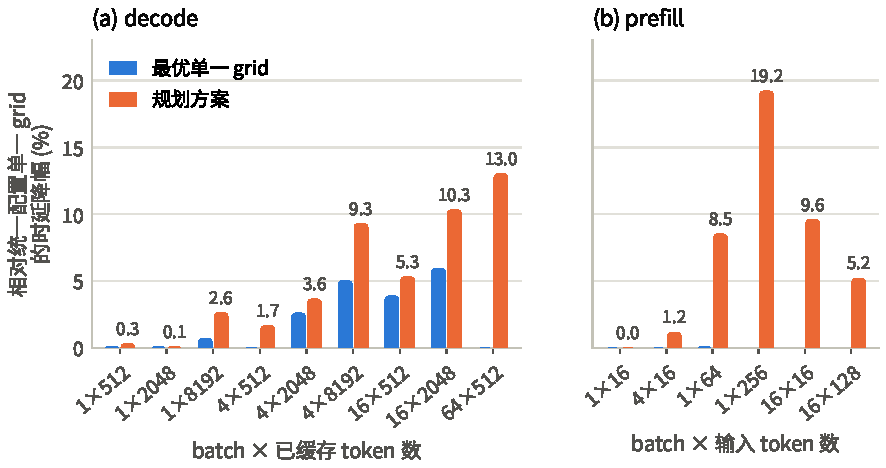
\includegraphics[width=\textwidth]{Img/midterm/gain}
\caption{15 个基准负载上最优单一 grid 与规划方案相对统一配置单一 grid 的端到端时延降幅对比。柱顶数字标注规划方案的总降幅，清晰区分核内分阶段活跃块控制与物理切分/PDL 各自的贡献。}\label{fig:gain}
\end{figure}

\begin{figure}[!htb]\centering
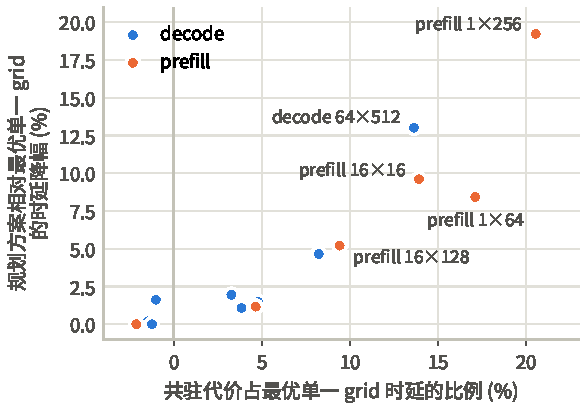
\includegraphics[width=0.66\textwidth]{Img/midterm/rule}
\caption{全网累计共驻代价占比与规划方案端到端收益的定量相关性（Spearman 秩相关系数 $\rho=0.92$）。}\label{fig:rule}
\end{figure}

\subsubsection{PDL 静态规则与引导式规划器验证}

首先检验静态 PDL 启用规则的端到端效果。在微观层面，decode $1\times 512$ 全切分五类边界的核内计时分解表明，PDL 将算子间等待间隙由 1.95--2.21\us 压缩至 0.67--0.78\us，扣除后继轻微负载不均增加的 0.4--0.8\us 后，每条边界净节省 0.58--0.80\us。在全部 16 组真实全切分方案上对比三种 PDL 策略（图~\ref{fig:rulereal}）：全局盲目开启导致 10 个方案慢于串行（最差 $-18.8\%$，中位数 $-0.45\%$）；本文提出的静态 PDL 规则在全部 16 组方案上实现零负向回退，中位加速 $+1.98\%$，与逐边实测贪心搜索（$+1.71\%$）相当。

\begin{figure}[!htb]\centering
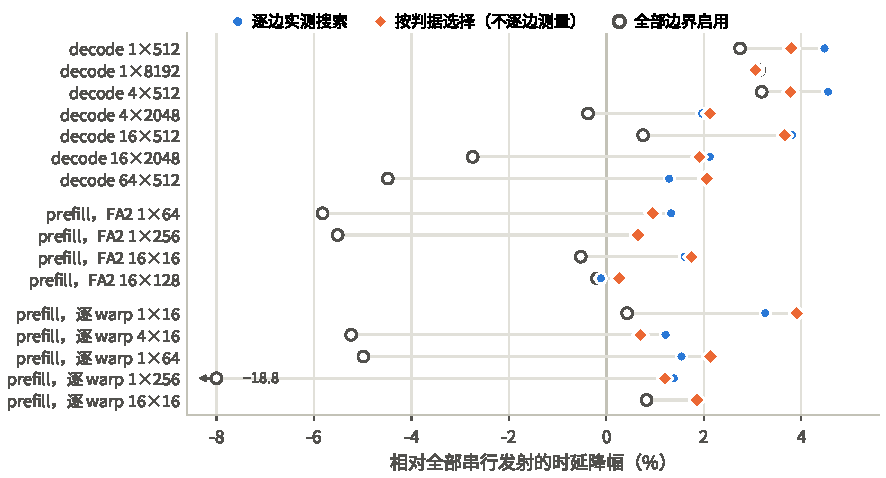
\includegraphics[width=\textwidth]{Img/midterm/v4_rulereal}
\caption{16 个真实模型全切分方案上三种 PDL 策略相对纯串行 completion 的端到端时延降幅对比。静态 PDL 规则在全部方案上均无负收益，整体表现与逐边实测搜索相当。}\label{fig:rulereal}
\end{figure}

其次检验模型与静态规则引导的离线规划器。图~\ref{fig:guided} 在全部 15 个基准负载上对比了引导式规划器与基准穷举规划器的测量开销与方案质量：引导式流程将分组配置实测次数压缩至穷举的 62\%、整网端到端实测次数压缩至 20\%，总测量量降至 43\%（单负载中位规划耗时由 40\,s 缩短至 21\,s，prefill $16\times 128$ 由 262\,s 降至 99\,s）；同时，报告集上的端到端时延偏差严格控制在 $\pm 1.0\%$ 以内（中位数 $-0.15\%$，峰值加速 19.6\%），验证了受控搜索空间规划的高效性与可靠性。

\begin{figure}[!htb]\centering
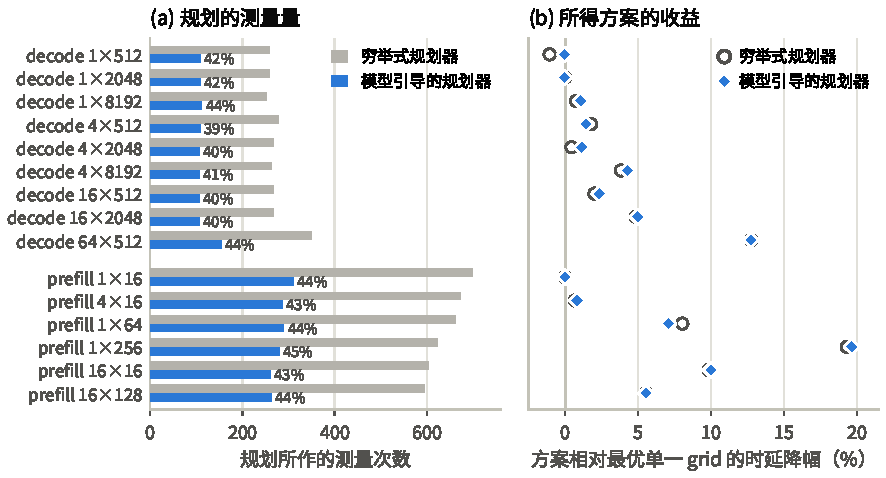
\includegraphics[width=\textwidth]{Img/midterm/v4_guided}
\caption{模型与静态规则引导规划器相对穷举规划器的测量开销缩减与端到端收益保持度。(a) 15 个基准负载上的总实测次数对比（条末百分比为引导式占穷举式的比例）；(b) 两种规划器选出方案在报告集上相对最优单一 grid 的时延降幅。}\label{fig:guided}
\end{figure}
